\documentclass{article}
\usepackage{caption}
\usepackage{subcaption}
\usepackage{comment}
\usepackage[a4paper,left=2.5cm,right=2.5cm,top=3.5cm,bottom=2.5cm]{geometry}
\usepackage{graphicx}

\usepackage[utf8]{inputenc}
\usepackage{makecell}
\usepackage{moresize}
\usepackage{multirow}
\usepackage{multicol}
\usepackage{natbib}
\usepackage{stmaryrd}
\usepackage{amsmath}
\usepackage[ruled,vlined]{algorithm2e}
\usepackage{fancyhdr}
\usepackage{graphicx}
\usepackage{paracol}
\usepackage[inline]{enumitem}
\usepackage{threeparttable}
\usepackage{amsfonts}
\usepackage{array}
% \usepackage{indentfirst}

\usepackage[hidelinks]{hyperref}
\usepackage{xcolor}
\definecolor{red}{HTML}{c81818}
\hypersetup{
    colorlinks=true,
    linkcolor=red,
    filecolor=magenta,      
    urlcolor=blue,
    citecolor={green!60!black}
}

\pagestyle{fancy}
\fancyhf{}
\rhead{Big Data Management}
\lhead{\textbf{Eindhoven University of Technology}}
\rfoot{\thepage}
\lfoot{Group 5}

\begin{document}

\begin{titlepage}
    \begin{center}
        
\includegraphics[width=0.6\textwidth]{tuelogo}
    
        \vspace*{1cm}
    
        {\huge \textbf{Distribution of Computation \&\\Experimental performance}}\\
        \vspace*{0.25cm}
        
        {\Large Big Data Management}\\
        
        \large{Milestone 2}
    
    \end{center}
    
    \vfill
       
    {\parindent0pt
        \textbf{Group 5}\\
        
        Çağla Sözen, 1597884\\
        c.sozen@student.tue.nl\\
        
        Gabriela Slavova, 1555855\\
        g.slavova@student.tue.nl\\
        
        Henrique Dias, 1531484\\
        h.a.coelho.dias@student.tue.nl\\
        
        Maria Pogodaeva, 1615556\\
        m.pogodaeva@student.tue.nl\\
        
        Nimo Beeren, 1019824\\
        n.beeren@student.tue.nl\\
        
        Panagiotis Banos, 1622773\\
        p.banos@student.tue.nl\\
        
        \vspace*{1cm}
    
        \textbf{Department of Mathematics and Computer Science}\\
        P.O.Box 513, MetaForum\\
        5612 AZ, 5600 MB Eindhoven\\
        The Netherlands
    }
\end{titlepage}

\section{Distribution of Computation}\label{sec:distribution}
    
    Let $R$ be a collection of records in a data set, ${A = \{a_1, a_2, ..., a_k, ...\}}$ be a set of its attributes. Let $S_A \subset A$ be a subset of up to 3 attributes from $A$ (i.e. $1 \leq |S_A| \leq 3$). For an arbitrary record $r\in R$, by $r.a_k$ we define a value of $a_k$ for $r$, and by $r.S_A$ a collection of values of attributes in $S_A$ for $r$.
    
    \subsection{Detecting Functional Dependencies}\label{sec:detection}
    
    First, we generate a set $H$ of all candidate functional dependencies (FDs) $S_A \rightarrow a_k$, on the central computer with a simple brute force algorithm. We proceed with a number of map and reduce steps.
    
    \paragraph{Common part.} 
    To detect any dependency, for each candidate FD $(S_A \rightarrow a_k) \in H$ we apply 4 steps:
    \setlist{nolistsep}
    \begin{enumerate}[noitemsep]
        \item \textbf{Map} each record $r \in R$ to a pair $((lhs, rhs), 1)$, with $lhs = r.S_A$ and $rhs=r.a_k$.
        
        \item \textbf{Reduce} all pairs $((lhs, rhs), 1)$ \textbf{by key} $(lhs, rhs)$, to a pair $((lhs, rhs), c)$ with $c$ the sum of their counts.
        
        \item \textbf{Map} each pair $((lhs, rhs), c)$ to a pair $(lhs, \{(rhs, c)\})$
        
        \item \textbf{Reduce} all pairs $(lhs, \{(rhs, c)\})$ \textbf{by key} $lhs$ to a pair $(lhs, S)$ with $S = \{(rhs_1, c_1), (rhs_2, c_2), ...\}$

    \end{enumerate}
    
    \paragraph{Hard and soft functional dependencies.}
    For hard and soft FDs, we compute the probability ${P_{FD} = \mathbb{P}(r_i.a_k = r_j.a_k \;|\; r_i.S_A = r_j.S_A)}$ for two randomly selected records $r_i, r_j \in R$, as follows:
    
    \begin{enumerate}[noitemsep]
        \setcounter{enumi}{4}
        \item \textbf{Map} each pair $(lhs, S)$ to a pair $(c_{t}, p)$, where $\displaystyle c_t = \sum_{(rhs,c) \in S} c$ is the total number of records $r \in R$ with $r.S_A = lhs$ and $\displaystyle p = \sum_{(rhs, c) \in S}\frac{c(c-1)}{c_t(c_t-1)}$ is the probability of randomly selecting two records $r_i, r_j$ with $r_i.a_k = r_j.a_k$ given $r_i.S_A = r_j.S_A = lhs$.
        
        \item \textbf{Map} each pair $(c_t, p)$ to a pair $(c_t, p_w)$, where $p_w = p\cdot c_t$ is the probability weighted by $c_t$
        
        \item \textbf{Reduce} all pairs $(c_t, p_w)$ to a pair $(C_t, P_w)$ where $C_t = \sum c_t$, $P_w = \sum p_w$
        
        \item \textbf{Map} each pair $(C_t, P_w)$ to the value $P_w / C_t$, which is the sought probability $P_{FD}$
    \end{enumerate}

    \noindent We can now classify $S_A \rightarrow a_k$ as hard if $P_{FD} = 1$ or soft if $P_{FD} \geq \tau$ for a given threshold $0 \leq \tau \leq 1$.
    
    \paragraph{\texorpdfstring{$\delta$}{delta}-functional dependencies.}
    For $\delta$-FDs, we use binary difference functions $\Delta$: the absolute difference relative to the full range for numerical attributes and the ratio of sequence similarity ($2M/T$ where $T$ is the total length of both sequences, and $M$ is the number of matches~\cite{difflib}) for string-valued attributes. After step 4 we apply:
    
    \begin{enumerate}[noitemsep]
        \setcounter{enumi}{4}
        \item \textbf{Map} each pair $(lhs, S)$ to a boolean value $X = \forall_{(rhs,c) \in S} \forall_{(rhs', c') \in S} : \Delta(rhs, rhs') \leq \delta$, for a given threshold $0 \leq \delta \leq 1$%.where $\delta$ is a given threshold, e.g. 0.05.
        \item \textbf{Reduce} all booleans $(X_1, X_2, ...)$ to a boolean value $X_1 \wedge X_2 \wedge ...$, which indicates whether the $\delta$-FD holds or not.
    \end{enumerate}
    
    % \noindent Finally, for all types of detected FDs if there exists an FD $S_A' \rightarrow a_k$ such that $S_A' \subset S_A$, we consider $S_A \rightarrow a_k$ as a \textbf{non-minimal} and thus we drop it.
    
    \subsection{Bottlenecks}\label{sec:bottlenecks}
    % PROBLEMS WE HAVE
    
        There are some specific parts of the algorithm that significantly influence its time complexity. We can refer to them as bottlenecks.
    
        \paragraph{Candidate set generation.}
        
        The set of candidate FDs $H$ grows exponentially with the number of attributes $|A|$. To be precise, when considering candidates with $k$ attributes on the left-hand side, the number of candidates is given by $\binom{|A|}{k+1}$. Thus, the generation of all candidates has a time complexity at least $\mathcal{O}(|A|!)$. Furthermore, in our implementation this procedure is executed centrally, so it cannot be sped up by adding more workers. However, for our dataset the time required to generate candidates is negligible compared to the time required to check the validity of these FDs.

        \paragraph{Sending candidates to workers.}
        
        After candidate set generation on the central machine, all candidate FDs must be sent to the workers. This communication overhead in Spark can take up to seconds for each candidate, depending on cluster characteristics.
        
        % As the candidate dependencies are calculated centrally, they need to be sent to Spark to distribute the rest of the execution. Our first approach was very straightforward, where we sent each candidate dependency to Spark one by one. Although the complete data set is sent to Spark at the beginning of execution, the data is distributed over different nodes and it needs to be fetched from all the nodes every time it's being accessed and the overhead for this is non-negligible. Depending on the architecture and the size of the cluster used, the overhead may be in the order of seconds. Even for smaller data sets with fewer attributes, initializing the verification of each functional dependency may take a considerable amount of time, and hence this overhead aggravates as the dataset size and number of attributes increase and this operation becomes the bottleneck for the execution. 
        
        \paragraph{$\Delta$-Comparisons.}
        
        Detecting $\delta$-functional dependencies requires computing the distance $\Delta(rhs, rhs')$ for all possible pairs of values $rhs, rhs'$ (see step 5 of the $\delta$-algorithm). It has a time complexity of  $\mathcal{O}(n^2)$ for numerical attributes and $\Omega(n*m)$ for string-typed attributes, where $n$ is the number of distinct values and $m$ is the length of the longest string being compared. %Therefore, detection of delta dependencies takes significantly more time than hard and soft dependencies. Hence, it is considered as a bottleneck operation. 
        
        \paragraph{Load imbalance.}
        
        Although the MapReduce paradigm ensures that the workload can be efficiently distributed over the cluster (some workers can start reducing while others are still at the mapping step), there is still a possibility of load imbalance if some nodes receive records with a significantly larger number of distinct values.\\
        
        \noindent To address some of these bottlenecks, several optimizations are implemented and discussed in \autoref{sec:optimizations}.

    % \subsection{Load Imbalance}
        % By applying the MapReduce paradigm, the algorithm can be efficiently distributed over a cluster of computers. The set of records is first partitioned and distributed over the workers. Then each worker starts counting values in the records it received. Because each reducer applies a commutative and associative function, the order in which elements are reduced does not matter. This allows some workers to start reducing while other workers are still at the previous mapping step. Furthermore, Spark will perform the reduction locally as much as possible, limiting communication cost.
    
        % However, there is still a possibility of load imbalance if some nodes receive records with a larger number of different values. This is because dealing with more values takes more time and as a consequence some node could be loaded more than others. Still, this depends on the way Spark distributes the records over the workers.

    \subsection{Optimizations}\label{sec:optimizations}
    % HOW WE ADDRESS THE DESCRIBED PROBLEMS
    
        \paragraph{Sending candidates to workers.}
        To address the bottleneck due to the overhead of sending candidate dependencies one by one to the workers, we partitioned the candidate dependency space and sent them in batches. The algorithm used for batching is explained below. This optimization decreased the run time from \textbf{4m37s} to \textbf{34s} on a small subset of the data.
        
        Let $H_i \subset H$ be a subset of candidate set with $i$ elements on the left-hand side, $i = \{1,2,3\}$.
        
        \begin{enumerate}[noitemsep]
            \item Run the FD Detection algorithm for $H_i$
            \item Generate $H_{i+1}$ and purge those FD that are non-minimal (see below)
            \item Partition filtered $H_{i+1}$ in subsets of given size \textit{chunk\_size} or as a whole if \textit{chunk\_size} is not specified.
            \item Run the FD Detection algorithm for all subsets
        \end{enumerate}
        
        % Let $C_iLHS$ be all candidates with i LHS elements and $i \in [1,3)$.
        
        % \begin{enumerate}[noitemsep]
        %     \item Run the FD Detection algorithm for all $C_iLHS$.
        %     \item Generate $C_{i+1}LHS$ and filter all minimal dependencies. (i.e remove from $C_{i+1}LHS$ all the supersets of dependencies found in $C_{i}LHS$). This yields, $C_{i+1}LHS\_Filtered$
        %     \item Partition $C_{i+1}LHS\_Filtered$ in subsets of size $|C_{i}LHS|$ (or an arbitrary \textit{chunk\_size} value).
        %     \item Run the algorithm for all subsets.
        % \end{enumerate}
        
        \paragraph{Purging Non-Minimal Functional Dependencies}
        To avoid running the FD detection algorithm redundantly for non-minimal FDs, given a list of candidate dependencies we purge the non-minimal ones before splitting the whole candidate list into a batch. Let $fd$ be an already detected FD and $cfd$ be the candidate FD, then if a candidate dependency satisfies the following formula, then its a non-minimal dependency: ${(fd.lhs) \subseteq (cfd.lhs) \wedge fd.rhs = cfd.rhs)}$

        \paragraph{$\Delta$-comparisons.} 
        
        First of all, since hard FD by definition also implies $\delta$-FD, we only check those candidates that \textit{have not yet been found hard}. Secondly, for numerical attributes is it enough to compute $\Delta(\max rhs, \min rhs)$ instead of pairwise comparisons, which decreases time complexity to $\mathcal{O}(n)$ where n is the number of records compared. Due to the nature of sequence matching technique, it is not possible to do the same for string attributes. Nevertheless, we can still optimize the process by using the \textit{upper bound} on similarity ratio~\cite{difflib}, and thus a \textit{lower bound} on difference ratio, which may produce false positives but no false negatives reducing the run time significantly. In this context, we can also use \textit{early stopping} on a single worker which allows stopping pairwise string comparisons as soon as we found one violating pair.

        \paragraph{Sampling.}
        
        % The computational cost of discovering FDs is determined by the number of records and the number of attributes of the dataset. More specifically it is ${\mathcal{O}(n^2\cdot(\frac{m}{2})^2\cdot2^m)}$ as shown by Liu et al\cite{liuFDComplexity}, where $n$ is the number of records $r$ in the database and $m$ is the number of attributes $a$. 
        Instead of scanning the whole dataset at once for detecting FD, we can benefit a lot from scanning a small sample first. It can significantly reduce $H$ for a relatively small computational cost. This optimization decreased the run time from \textbf{6m30s} to \textbf{2m30s} on a subset of the data. However it should be noted that this produces and approximation of the real FDs, therefore this might result in some false negatives for soft FDs.
        
        To perform the sampling we implement the following steps:
        
        \begin{enumerate}[noitemsep]
            \item Create $n$ subsets of $R$ of by performing random uniform sampling without replacement such that $R_i \subseteq R$ and $\forall i \in [1,n]$. The size of the subsets is determined by a sampling ratio $0 \leq r \leq 1$ such that $|R_i| = r |R|$ for all $i$. The smaller the sampling ratio, the less accurate the approximation becomes.
            
            \item For each subset $R_i$ calculate the set of candidate $H_i$ and maintain only the FDs whose $P_{FD}$ surpasses a given threshold $0 \leq s \leq 1$ along with the delta candidates due to the necessity of going over all candidates for detecting $\delta$-dependencies by definition.
            
            \item Obtain the intersection of candidate subsets $H = H_1\cap H_2 \cap \ldots \cap H_n$ to find the shared FD candidates.
            
            \item Compute the FDs of the full dataset $R$ with respect to set $H$.
        \end{enumerate}
        
        \paragraph{Excluded Potential Optimizations} 
        
        On the other hand, there were some optimization ideas that have been discussed but didn't end up in the final implementation. One of them was to use early stopping workers simultaneously while detecting the FDs, according to the detection of another. To implement this we need to send a signal to all individual workers once one of them has encountered a violation. This task requires using a \textit{Spark Listener} to keep track of and to manipulate callbacks~\cite{spark_doc}. However, unlike Java and Scala, PySpark does not yet provide this functionality, and hence we weren't able to implement this feature \cite{spark_doc_sched}.
        
        Furthermore, following from the same idea of early stopping  for the $\delta$-dependencies, we can stop checking the candidates for hard FD as soon as $|S| > 1$ at step 4 of the algorithm. However since we search for hard and soft FD at the same time, we do not stop by this condition. The advantages of using one procedure for both types of FD outweighs the advantages of early stopping here.
        
        Finally, no optimizations were implemented for candidate set generation and load imbalance because a bruteforce algorithm was used to detect functional dependencies and the efficiency of this algorithm was not the focus of the project. Furthermore, load balancing could be optimized by manually scheduling loads distributed over the workers however, PySpark API does not yet provide control over concurrent jobs. 
    
        
        % \paragraph{Early Stopping:} When detecting hard- or $\delta$-FDs, we can use an early stopping technique where we stop the computation as soon as we find two distinct values for the right-hand side values for the same left-hand side value. This can be applied in step 5 of the described algorithm by stopping if $|S| > 1$. Since we look for hard and soft FDs at the same time, this optimization is not used for those kinds of dependencies. By definition, presence of a hard dependency implies  presence of a delta dependency. On the other hand, since the presence of a soft dependency does not affect the presence of a $\delta$ dependency, the algorithm continues with the detection of delta dependencies subsequently. Therefore, this optimization could save time in theory for the detection of $\delta$ dependencies. 
        
        % This optimization however requires having control over the workers individually to be able to signal other workers to stop once a value violating the dependency is found in one of the workers. Although this capability can be achieved by partitioning the data according the number of available cores, reusing the same RDD multiple times on the same set of workers and manually synchronizing multi-threaded execution for the proper distribution of tasks on the workers, it's not a trivial task and requires using a \textit{Spark Listener} to keep track of and to manipulate callbacks~\cite{spark_doc}. However, unlike Java and Scala, PySpark does not yet provide this functionality therefore early stopping has not been implemented as part of the optimizations for this project. Instead, a similar alternative was used which will be discussed under the proceeding subtitle. 
        
\section{Experimental Performance \& Scalability}

    \subsection{Dataset Properties}
    To measure the scalability of our program we varied the number of records and number of attributes of the dataset. On \autoref{fig:plot records} we can see how the execution time increases with the increasing number of records. Since the complexity of $\Delta$-comparisons is quadratic in the number of unique values, we would expect running time to increase quadratically with the number of rows. With our data, we cannot confidently reject this hypothesis, but scalability was sufficient for our use case. The execution time is expected to grow exponentially with the number of attributes, and as shown in \autoref{fig:plot attrs} we found no evidence to reject this hypothesis. For measurements with $>$ 13 attributes, additional data was generated.
    
    \subsection{System Properties}
    With respect to the system properties we tried variants with different number of CPU threads and cluster nodes. On \autoref{fig:plot cpus} we can see that on a local machine with only 2 cores the execution time is significantly larger than when the system has 4 cores. This is to be expected as the work is less distributed since there are less workers. On the cluster we see that increasing the number of workers does not decrease the execution time significantly. At this point, the additional computational power is outweighed by the communication overhead for our solution.
    
    \subsection{Sampling}
    
    We also tried testing how performing sampling and approximating the FDs change the execution time. On \autoref{fig:plot sampling ratio} we can see the clear difference in execution time between the runs with and without sampling. Using this technique drops the execution time by half. It is clear that this optimization is very effective and useful for approximations. Finally, run time increases once again as the sampling ratio increase since a large portion of the data is sampled and scanned several times.  

    \begin{figure}
        \centering
        \begin{subfigure}[t]{0.45\textwidth}
            \centering
            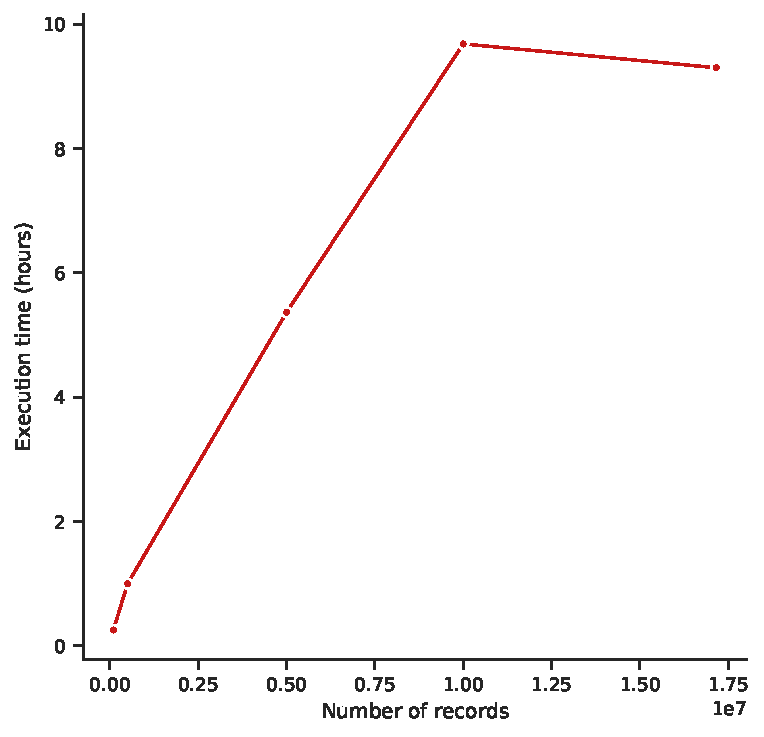
\includegraphics[width=\textwidth]{figures/plot_num_records.pdf}
            \caption{Scalability over number of records. All jobs were executed on a cluster of 24 workers and 1 master node with 4 threads and 15 GB memory each.}
            \label{fig:plot records}
        \end{subfigure}
        \hfill
        \begin{subfigure}[t]{0.45\textwidth}
            \centering
            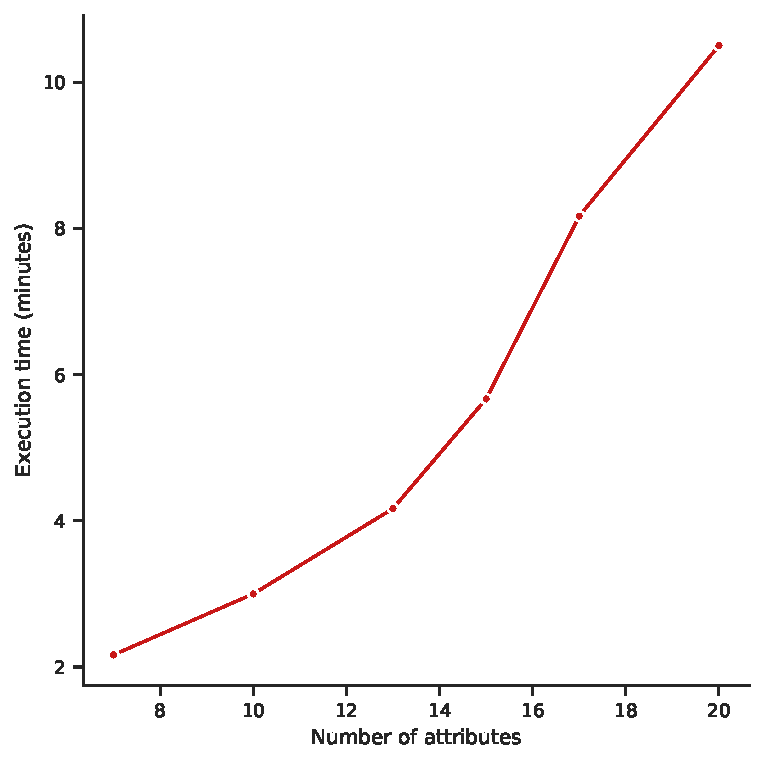
\includegraphics[width=\textwidth]{figures/plot_num_attrs.pdf}
            \caption{Scalability over number of attributes. All jobs were executed on a single machine with 4 threads and 16 GB of memory.}
            \label{fig:plot attrs}
        \end{subfigure}
        
        \medskip
        
        \begin{subfigure}[t]{0.45\textwidth}
            \centering
            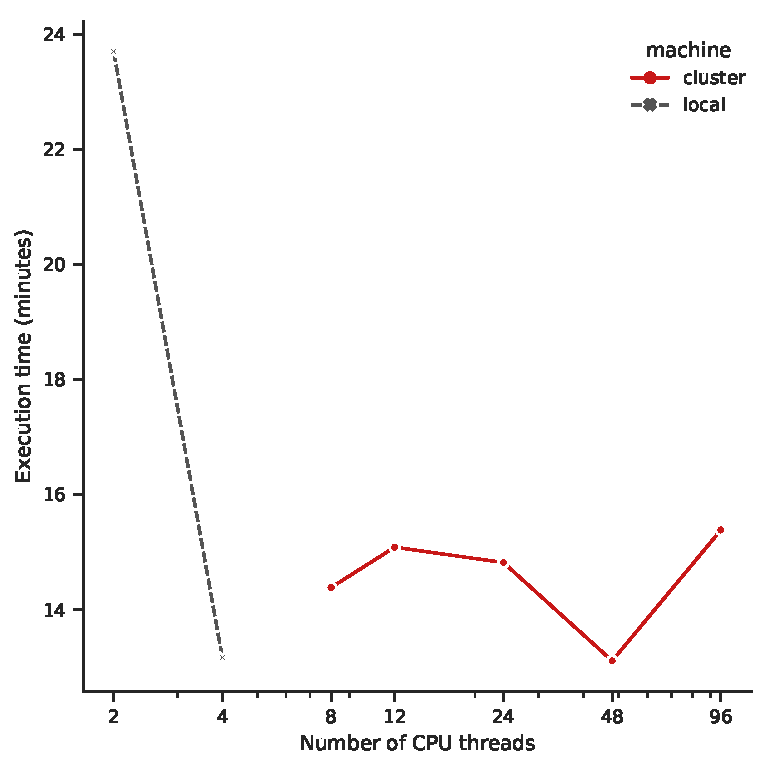
\includegraphics[width=\textwidth]{figures/plot_num_cpus.pdf}
            \caption{Scalability over number of CPU threads. The series of cluster jobs were executed on $n$ workers and 1 master node with 15 GB memory each, where $n = \text{\#threads}/4$. The series of local jobs were executed on a single machine with 16 GB of memory.}
            \label{fig:plot cpus}
        \end{subfigure}
        \hfill
        \begin{subfigure}[t]{0.45\textwidth}
            \centering
            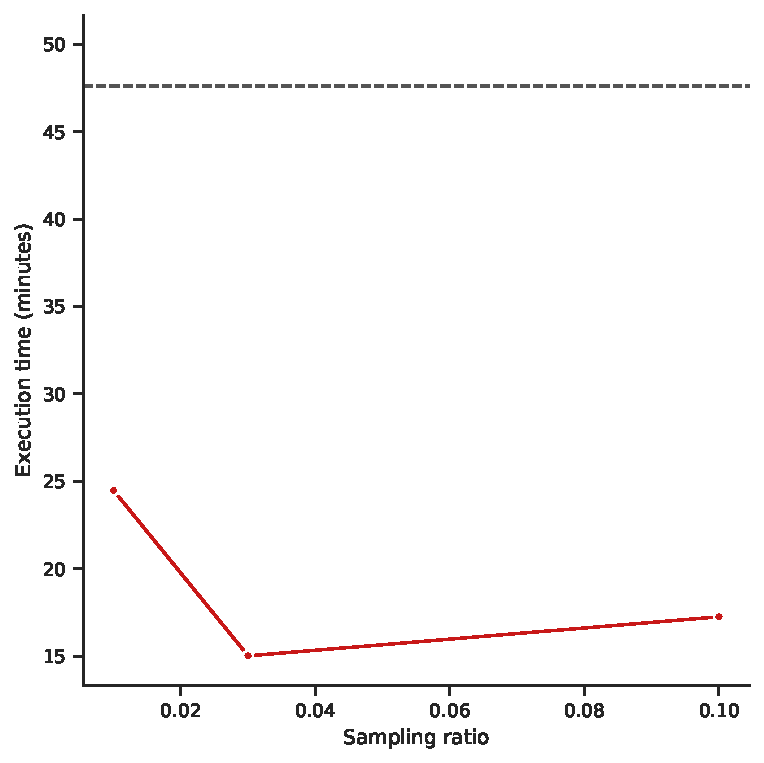
\includegraphics[width=\textwidth]{figures/plot_sampling_ratio.pdf}
            \caption{Effect of sampling ratio on execution time. The dashed line indicates the execution time without sampling. All jobs were executed on a single machine with 8 threads and 16 GB of memory.}
            \label{fig:plot sampling ratio}
        \end{subfigure}
        \caption{Running time as a function of various dataset properties and system properties. When not mentioned, the number of attributes is 13 and the number of records is 100,000.}
        \label{fig:three graphs}
    \end{figure}

\section{Detected Dependencies} 

    \subsection{Detected}
    
    We ran our algorithm on the full dataset with $\tau = 0.75$, $\delta = 0.45$ and $r = 0.03$. All detected dependencies can be found in \autoref{tab:detected-fds}. We detected at least one of each type of dependency, but we had to set $\delta$ quite high to achieve this. As a result, the $\delta$-dependency $\texttt{location} \rightarrow \texttt{type}$ was found. However, this is only due to the fact that the \texttt{type} attribute has only two distinct values \texttt{ORG} and \texttt{USR}, which are within the $\delta$-threshold according to our string distance measure. Furthermore, the only hard dependency found was manually introduced by introducing the \textit{country\_code} attribute.  
    
        \begin{table}[ht]
            \centering
            \begin{tabular}{|p{0.07\textwidth}|p{0.3\textwidth}|}
                \hline
                \textbf{Type} & \textbf{Dependency} \\ %& %\textbf{Description} \\
                \Xhline{2\arrayrulewidth}
                Hard & $\texttt{country\_code} \rightarrow \texttt{country}$ \\ %& The country code is mapped to a unique country name.\\
                \hline
                $\delta$ & $\texttt{location} \rightarrow \texttt{type}$ \\
                \hline
                $\delta$ & $\texttt{state} \rightarrow \texttt{type}$ \\
                \hline
                $\delta$ & $\texttt{deleted} \rightarrow \texttt{type}$ \\
                \hline
                $\delta$ & $\texttt{company} \rightarrow \texttt{type}$ \\
                \hline
                $\delta$ & $\texttt{country\_code} \rightarrow \texttt{country}$ \\
                \hline
                $\delta$ & $\texttt{country\_code} \rightarrow \texttt{type}$ \\
                \hline
                $\delta$ & $\texttt{city} \rightarrow \texttt{type}$ \\
                \hline
                Soft & $\texttt{state} \rightarrow \texttt{country}$ \\ 
                \hline
                Soft & $\texttt{state} \rightarrow \texttt{deleted}$ \\ 
                \hline
                Soft & $\texttt{state} \rightarrow \texttt{type}$ \\ 
                \hline
                Soft & $\texttt{country} \rightarrow \texttt{company}$ \\ 
                \hline
                Soft & $\texttt{country} \rightarrow \texttt{longitude}$ \\
                \hline
                Soft & $\texttt{country} \rightarrow \texttt{location}$ \\ 
                \hline
                Soft & $\texttt{country\_code} \rightarrow \texttt{latitude}$ \\ 
                \hline
                Soft & $\texttt{country\_code} \rightarrow \texttt{longitude}$ \\ 
                \hline
                Soft & $\texttt{location} \rightarrow \texttt{type}$ \\ 
                \hline
                Soft & $\texttt{location} \rightarrow \texttt{city}$ \\ 
                \hline
                Soft & $\texttt{location} \rightarrow \texttt{latitude}$ \\ 
                \hline
                Soft & $\texttt{location} \rightarrow \texttt{longitude}$ \\ 
                \hline
                Soft & $\texttt{location} \rightarrow \texttt{company}$ \\ 
                \hline
                Soft & $\texttt{location} \rightarrow \texttt{state}$ \\
                \hline
                Soft & $\texttt{location} \rightarrow \texttt{deleted}$ \\ 
                \hline
                Soft & $\texttt{location} \rightarrow \texttt{country}$ \\ 
                \hline
                Soft & $\texttt{deleted} \rightarrow \texttt{type}$ \\ 
                \hline
                Soft & $\texttt{city} \rightarrow \texttt{country}$ \\ 
                \hline
                Soft & $\texttt{country} \rightarrow \texttt{city}$ \\ 
                \hline
                Soft & $\texttt{country\_code} \rightarrow \texttt{deleted}$ \\ 
                \hline
                Soft & $\texttt{company} \rightarrow \texttt{type}$ \\ 
                \hline
                Soft & $\texttt{type} \rightarrow \texttt{state}$ \\ 
                \hline
                Soft & $\texttt{type} \rightarrow \texttt{city}$ \\ 
                \hline
                
                
                %& Most states only exist in a single country. However, the dependency is not hard since a null value of \texttt{state} may be associated with different countries.\\
                % \hline
                % Soft & $\texttt{city} \rightarrow \texttt{country}$ & Most city names only appear in one country, but some appear in multiple.\\
                % \hline
                % Soft & $\texttt{city} \rightarrow \texttt{state}$ & Most city names only appear in one state, but some appear in multiple.\\
                % \hline
                % Soft & $\texttt{company} \rightarrow \texttt{country}$ & For most companies, the majority of employees live in the same country.\\
                % \hline
                %& A single city covers a limited range of coordinates. The country is included on the left-hand side to deal with equal-named cities in different countries.\\
            \end{tabular}
            \quad
            \begin{tabular}{|p{0.07\textwidth}|p{0.3\textwidth}|}
                \hline
                \textbf{Type} & \textbf{Dependency} \\ %& %\textbf{Description} \\
                \Xhline{2\arrayrulewidth}
                
                Soft & $\texttt{type} \rightarrow \texttt{deleted}$ \\ 
                \hline
                Soft & $\texttt{company} \rightarrow \texttt{location}$ \\ 
                \hline
                % Soft & $\texttt{city} \rightarrow \texttt{country\_code}$ \\ 
                % \hline
                Soft & $\texttt{company} \rightarrow \texttt{state}$ \\ 
                \hline
                Soft & $\texttt{country} \rightarrow \texttt{state}$ \\ 
                \hline
                Soft & $\texttt{state} \rightarrow \texttt{company}$ \\ 
                \hline
                Soft & $\texttt{state} \rightarrow \texttt{location}$ \\ 
                \hline
                Soft & $\texttt{state} \rightarrow \texttt{city}$ \\ 
                \hline
                Soft & $\texttt{state} \rightarrow \texttt{latitude}$ \\ 
                \hline
                Soft & $\texttt{state} \rightarrow \texttt{longitude}$ \\ 
                \hline
                Soft & $\texttt{state} \rightarrow \texttt{country\_code}$ \\ 
                \hline
                Soft & $\texttt{company} \rightarrow \texttt{latitude}$ \\ 
                \hline
                Soft & $\texttt{company} \rightarrow \texttt{country}$ \\ 
                \hline
                Soft & $\texttt{company} \rightarrow \texttt{deleted}$ \\ 
                \hline
                Soft & $\texttt{company} \rightarrow \texttt{city}$ \\ 
                \hline
                % Soft & $\texttt{company} \rightarrow \texttt{country\_code}$ \\ 
                % \hline
                Soft & $\texttt{city} \rightarrow \texttt{type}$ \\ 
                \hline
                Soft & $\texttt{city} \rightarrow \texttt{latitude}$ \\ 
                \hline
                Soft & $\texttt{city} \rightarrow \texttt{state}$ \\ 
                \hline
                Soft & $\texttt{city} \rightarrow \texttt{deleted}$ \\ 
                \hline
                Soft & $\texttt{city} \rightarrow \texttt{location}$ \\ 
                \hline
                Soft & $\texttt{city} \rightarrow \texttt{company}$ \\ 
                \hline
                Soft & $\texttt{city} \rightarrow \texttt{longitude}$ \\ 
                \hline
                Soft & $\texttt{deleted} \rightarrow \texttt{city}$ \\ 
                \hline
                Soft & $\texttt{country} \rightarrow \texttt{country\_code}$ \\ 
                \hline
                Soft & $\texttt{country\_code} \rightarrow \texttt{company}$ \\ 
                \hline
                Soft & $\texttt{country\_code} \rightarrow \texttt{state}$ \\ 
                \hline
                Soft & $\texttt{country\_code} \rightarrow \texttt{location}$ \\ 
                \hline
                Soft & $\texttt{country\_code} \rightarrow \texttt{city}$ \\ 
                \hline
                Soft & $\texttt{country} \rightarrow \texttt{deleted}$ \\ 
                \hline
                Soft & $\texttt{deleted} \rightarrow \texttt{state}$ \\ 
                \hline
                Soft & $\texttt{country} \rightarrow \texttt{latitude}$ \\ 
                \hline
                Soft & $\texttt{country} \rightarrow \texttt{type}$ \\ 
                \hline
                Soft & $\texttt{type} \rightarrow \texttt{company}$ \\ 
                \hline
                
                % Soft & $\texttt{location} \rightarrow \texttt{country\_code}$ \\ 
                % \hline

                
                
            \end{tabular}
            \caption{Detected functional dependencies}
            \label{tab:detected-fds}
        \end{table}
    
    \subsection{Expected but not Detected Dependencies}
    
    There were some dependencies that were  expected but not detected, which can be found alongside an explanation in \autoref{tab:not-detected-fds}.
    
        \begin{table}[!h]
            \centering
            \begin{tabular}{|p{0.07\textwidth}|p{0.3\textwidth}|p{0.55\textwidth}|}
                \hline
                \textbf{Type} & \textbf{Dependency} & \textbf{Explanation} \\
                \Xhline{2\arrayrulewidth}
                Hard & $\texttt{country} \rightarrow \texttt{country\_code}$ & This FD was found to be soft, which can be explained by two different country codes being mapped to a null value (because they were not recognized as an ISO-3166 country code).\\
                \hline
                Soft & $\texttt{company}, \texttt{country} \rightarrow \texttt{city}$ & This FD was violated in one of the samples, and so was not checked on the full dataset. However, that does necessarily mean that it would not be a soft FD on the full dataset.\\
                \hline
                $\delta$ & $\texttt{city}, \texttt{country} \rightarrow \texttt{long}, \texttt{lat}$ & This $\delta$-FD was violated because of null values on the \texttt{city} attribute.\\      \hline
                % Soft & $\texttt{state} \rightarrow \texttt{country}$ & Most states only exist in a single country. However, the dependency is not hard since a null value of \texttt{state} may be associated with different countries.\\
                % \hline
                % Soft & $\texttt{city} \rightarrow \texttt{country}$ & Most city names only appear in one country, but some appear in multiple.\\
                % \hline
                % Soft & $\texttt{city} \rightarrow \texttt{state}$ & Most city names only appear in one state, but some appear in multiple.\\
                % \hline
                % Soft & $\texttt{company} \rightarrow \texttt{country}$ & For most companies, the majority of employees live in the same country.\\
                % \hline
                % $\delta$ & $\texttt{city}, \texttt{country} \rightarrow \texttt{long}, \texttt{lat}$ & A single city covers a limited range of coordinates. The country is included on the left-hand side to deal with equal-named cities in different countries.\\
                % \hline
            \end{tabular}
            \caption{Expected but not detected functional dependencies}
            \label{tab:not-detected-fds}
        \end{table}

\clearpage
\appendix
\section{Appendix}\label{appendix}
    \subsection{Team Contribution}
     
    \begin{table}[ht]
    \centering
        \begin{tabular}{|p{0.2\textwidth}|p{0.2\textwidth}|p{0.52\textwidth}|}
        \hline
        \textbf{Student Name} & \textbf{Contribution (\%)} & \textbf{Participation in Tasks} \\
        \Xhline{2\arrayrulewidth}
        
        Çağla Sözen & $16.\overline{6}\%$ & Testing, Early stopping, candidate space partitioning research,  writing the report, preparing the poster, recording the video.\\
        \hline
        
        Gabriela Slavova & $16.\overline{6}\%$ & Candidate space partitioning research, experimental results \& scalability, writing the video script, writing the report.\\
        \hline
        
        Henrique Dias & $16.\overline{6}\%$ & Candidate space partitioning research \& implementation, discarding non-minimal FDs, adapting code for HPC, running code on HPC, writing the report.\\
        \hline
        
        Maria Pogodaeva & $16.\overline{6}\%$ & $\delta$-FDs implementation, reduced $\delta$-FDs implementation, writing the report.\\
        \hline
        
        Nimo Beeren & $16.\overline{6}\%$ & $\delta$-FDs implementation, reduced $\delta$-FDs implementation, code refactoring, experimental performance \& scalability, running code on HPC, writing the report. \\
        \hline
        
        Panagiotis Banos & $16.\overline{6}\%$ & Early stopping, sampling implementation, writing the report, preparing the poster. \\
        \hline
        
        \end{tabular}
        \caption{Team Contribution}
        \label{tab:contribution}
    \end{table}
    
    Every team member is involved in the project, approaches the tasks responsibly and shows interest. Mostly our work is conducted as a team effort during the meetings, in addition to that we also try to distribute separate tasks among the team members.
    
    
\newpage

% if we want to sort the links in alphabetical order:
\bibliographystyle{plain}
% if we want to sort the links as they appear in the text:
% \bibliographystyle{unsrt}
\bibliography{references}

\end{document}